\documentclass[twocolumn,oneside,a4paper,12.0pt]{article}
% ---------------- Para Modificar ---------------- 
\newcommand{\principal}{Volumes}
\newcommand{\conteudo}{}
\newcommand{\turmas}{3~EMSI~A e do 3~EMSI~B}

\date{abril de 2021}

\newcommand{\citacao}{Que nada nos defina. Que nada nos sujeite. Que a liberdade seja a nossa própria substância.}
\newcommand{\autorcitacao}{Simone de Beauvoir}
% ------------------------------------------------

%-------------------------------------------------
\usepackage[english,brazilian]{babel}
\usepackage[alf]{abntex2cite}
\usepackage[utf8]{inputenc}
\usepackage[T1]{fontenc}
\usepackage[top=15mm, bottom=15mm, left=10mm, right=10mm]{geometry}
\usepackage{framed,booktabs,color,hyperref,graphicx}
\usepackage{amsfonts,amsthm,cancel}
\usepackage{subfigure,enumerate,float}
  
\definecolor{shadecolor}{rgb}{0.8,0.8,0.8}
\pagenumbering{arabic}

% Colunas
\usepackage{multicol}
\columnsep=10mm %Espaçamento entre colunas.
\setlength{\columnseprule}{1pt}

% Cabeçalho
\usepackage{fancyhdr}
\pagestyle{fancy}
\lhead{\textbf{\principal}}
\rhead{}
\renewcommand{\headrulewidth}{1pt} % espessura da linha do cabeçalho
\renewcommand{\footrulewidth}{1pt} % espessura da linha do rodapé

% Parágrafo
\setlength{\parindent}{1.25cm}

\newtheorem{problema}{Problema}
\newtheorem{exercicio}{exercicio}
\newtheorem{exemplo}{Exemplo}
\newtheorem{questao}{Questão}

\usepackage[skip=10pt]{caption}
\captionsetup{font={stretch=0.4,small}}

\newcommand{\FRASE}{\textit{``\citacao ''}\\(\textbf{\autorcitacao})}

\title{\LINHAHORIZONTAL \\\textbf{\\ \principal}\footnote{Resumo para os estudos das aulas não presenciais no período de quarentena para as turmas do \turmas .}\\\LINHAHORIZONTAL}

\newcommand{\LINHAHORIZONTAL}{\center \rule{16cm}{1.25pt}}
\newcommand{\sol}{\textbf{Solução}}

\newcommand{\m}[1]{\(\displaystyle {#1}\)}
\newcommand{\M}[1]{\[{#1}\]}

\author{\textbf{Professor Leandro Vieira}\\EREM Regina Pacis\\Palmeirina-PE}
\newcommand{\frase}{\begin{verse} \flushright{\FRASE} \end{verse}}


\begin{document}
%%%%%%%%%%%%%%%%%%%%%%%%%%%%%%%%%%%%%%%%%%%%%%%%%%%%%%%%%%%%%%%%%%%%%%%%%%%%%%%%%%%
\section*{Exercícios Áreas}
% ==============================================================
\begin{enumerate}
\item A planificação abaixo é a representação de uma caixa de papelão.

	\begin{figure}[!htb]
	\center
	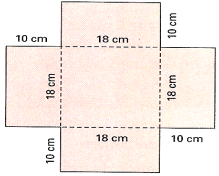
\includegraphics[width=7cm]{Extras/a1.png}
	\end{figure}

Quantos centímetros quadrados de papelão foram gastos para fazer a caixa?
	
	\begin{enumerate}
	\item 324 cm$^2$
	\item 360 cm$^2$
	\item 720 cm$^2$ 
	\item 1044 cm$^2$ 
	\item 2000 cm$^2$
	\end{enumerate}

% ==============================================================
\item Para economizar papelão, um fabricante de sabão em pó mudou as dimensões da embalagem de 1 Kg. As duas embalagens têm o formato de um paralelepípedo retângulo e suas dimensões estão indicadas no desenho abaixo.

	\begin{figure}[!htb]
	\center
	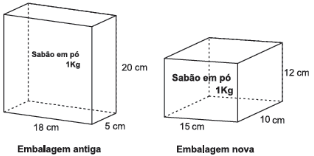
\includegraphics[width=7cm]{Extras/a2.png}
	\end{figure}

Considerando-se as medidas dadas e apenas a área externa das caixas, a economia de papelão que essa mudança resultou para a empresa, por caixa, foi de
	\begin{enumerate}
	\item 12 cm$^2$
	\item 60 cm$^2$
	\item 100 cm$^2$
	\item 200 cm$^2$
	\end{enumerate}

% ==============================================================
\item O desenho abaixo representa o pátio de um supermercado, onde foram construídas duas áreas para estacionamento e, no espaço restante, um jardim.

	\begin{figure}[!htb]
	\center
	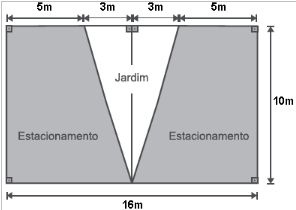
\includegraphics[width=7cm]{Extras/a3.png}
	\end{figure}

Qual é a medida da área total destinada ao estacionamento desse supermercado?

	\begin{enumerate}
	\item 65 m$^2$
	\item 80 m$^2$
	\item 130 m$^2$
	\item 160 m$^2$
	\item 210 m$^2$
	\end{enumerate}

% ==============================================================

\item Um reservatório cilíndrico de raio da base 3 m e altura 7 m, tem área da superfície lateral igual a

\begin{enumerate}
\item 42 $\pi m^2$.
\item 35 $\pi m^2$.
\item 32 $\pi m^2$.
\item 21 $\pi m^2$.
\item 18 $\pi m^2$.
\end{enumerate}

% ==============================================================

\item O desenho abaixo é formado por dois círculos concêntricos.  

	\begin{figure}[!htb]
	\center
	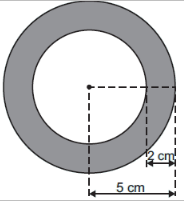
\includegraphics[width=7cm]{Extras/a4.png}
	\end{figure}

Qual é a medida da área da parte colorida de cinza?

\begin{enumerate}
\item 34 cm$^2$
\item 25 cm$^2$
\item 21 cm$^2$
\item 16 cm$^2$
\item 13 cm$^2$ 
\end{enumerate}

% ==============================================================

\item Uma empresa de publicidade utiliza dois tipos de suportes rotatórios para veicular propaganda, um em forma de cilindro circular reto de diâmetro 1 m e o outro em forma de um prisma reto, cuja base é um triângulo equilátero de lado medindo 1 m. Os dois suportes têm 5 m de altura, conforme indicado no desenho abaixo.

	\begin{figure}[!htb]
	\center
	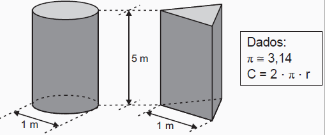
\includegraphics[width=7cm]{Extras/a5.png}
	\end{figure}

O preço cobrado por propaganda é de R\$ 100,00 por m2 de área lateral externa do suporte utilizado.	O valor a ser pago pela opção de suporte mais econômica para um anunciante é, aproximadamente,
	
\begin{enumerate}
\item R\$ 1 500,00
\item R\$ 1 570,00
\item R\$ 1 586,60
\item R\$ 1 727,00 
\end{enumerate}

% ==============================================================

\item Fábio construiu, em sua fazenda, um silo para armazenar soja. A parede cilíndrica desse silo será revestida com uma camada de manta. A figura abaixo representa o silo construído por Fábio com suas dimensões indicadas.

	\begin{figure}[!htb]
	\center
	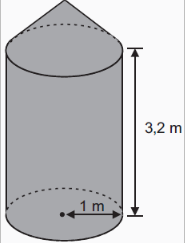
\includegraphics[width=7cm]{Extras/a6.png}
	\end{figure}

A quantidade mínima de manta, em metros quadrados, que Fábio deverá comprar para revestir a parte cilíndrica desse silo é 

\begin{enumerate}
\item 1,6 $\pi$. 
\item 2,0 $\pi$. 
\item 3,2 $\pi$. 
\item 6,4 $\pi$. 
\item 8,4 $\pi$. 
\end{enumerate}

% ==============================================================

\item 

	\begin{figure}[!htb]
	\center
	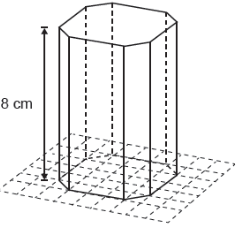
\includegraphics[width=7cm]{Extras/v3.png}
	\end{figure}


\begin{enumerate}
\item 
\end{enumerate}



% ==============================================================

\item 

	\begin{figure}[!htb]
	\center
	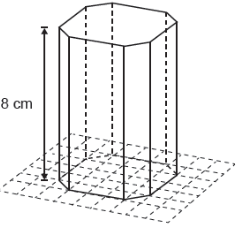
\includegraphics[width=7cm]{Extras/v3.png}
	\end{figure}


\begin{enumerate}
\item 
\end{enumerate}



% ==============================================================

\item 

	\begin{figure}[!htb]
	\center
	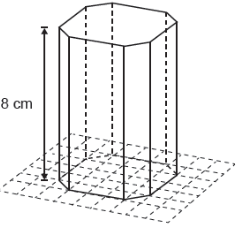
\includegraphics[width=7cm]{Extras/v3.png}
	\end{figure}


\begin{enumerate}
\item 
\end{enumerate}



% ==============================================================

\item 

	\begin{figure}[!htb]
	\center
	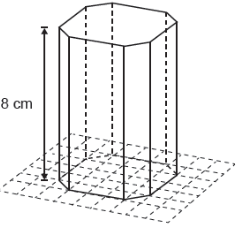
\includegraphics[width=7cm]{Extras/v3.png}
	\end{figure}


\begin{enumerate}
\item 
\end{enumerate}


% ==============================================================

\item 

	\begin{figure}[!htb]
	\center
	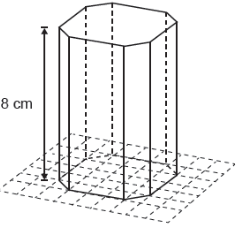
\includegraphics[width=7cm]{Extras/v3.png}
	\end{figure}


\begin{enumerate}
\item 
\end{enumerate}

\end{enumerate}
%%%%%%%%%%%%%%%%%%%%%%%%%%%%%%%%%%%%%%%%%%%%%%%%%%%%%%%%%%%%%%%%%%%%%%%%%%%%%%%%%%%
\section*{Exercícios Volumes}
\begin{enumerate}	
% ==============================================================
\item Alguns objetos, durante a sua fabricação, necessitam passar por um processo de resfriamento. Para que isso ocorra, uma fábrica utiliza um tanque de resfriamento, como mostra a figura.

	\begin{figure}[!htb]
	\center
	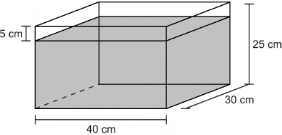
\includegraphics[width=7cm]{Extras/v1.png}
	\end{figure}

O que aconteceria com o nível da água se colocássemos no tanque um objeto cujo volume fosse de 2.400 cm$^3$? 	

	\begin{enumerate}
	\item O nível subiria 0,2 cm, fazendo a água ficar com 20,2 cm de altura. 
	\item O nível subiria 1 cm, fazendo a água ficar com 21 cm de altura. 
	\item O nível subiria 2 cm, fazendo a água ficar com 22 cm de altura. 
	\item O nível subiria 8 cm, fazendo a água transbordar. 
	\item O nível subiria 20 cm, fazendo a água transbordar.
	\end{enumerate}

% ==============================================================
\item Um recipiente cilíndrico cujo diâmetro da base é igual a 12 cm contém água até certa altura. Sofia colocou uma esfera de chumbo no interior do recipiente, que ficou totalmente submersa, e a altura da água desse recipiente subiu 1 cm. Qual é o raio dessa esfera?

	\begin{enumerate}
	\item 2,0 cm
	\item 3,0 cm
	\item 3,5 cm
	\item 4,5 cm
	\end{enumerate}

% ==============================================================
\item Um produtor de leite armazena seu produto em caixas com a forma de bloco retangular com altura de 25 cm e capacidade de 1 litro. Ele deseja trocar as caixas por embalagens em forma de cilindro, de mesma altura e mesma capacidade. Para que isso ocorra, o raio da base dessa embalagem cilíndrica, em cm, deve ser igual a

	\begin{enumerate}
	\item $ \sqrt{\frac{40}{\pi}} $
	\item $ \sqrt{\frac{60}{\pi}} $
	\item $ \sqrt{\frac{120}{\pi}} $
	\item $ \sqrt{\frac{160}{\pi}} $	
	\end{enumerate}

% ==============================================================
\item  A figura abaixo representa uma caixa de sapatos no formato de um prisma retangular que possui 30 cm de comprimento, 20 cm de largura e 10 cm de altura.

	\begin{figure}[!htb]
	\center
	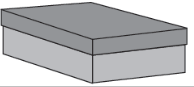
\includegraphics[width=7cm]{Extras/v2.png}
	\end{figure}

Qual é a capacidade máxima dessa caixa de sapatos? 

	\begin{enumerate}
	\item 50 cm$^3$
	\item 60 cm$^3$
	\item 600 cm$^3$
	\item 5 000 cm$^3$
	\item 6 000 cm$^3$
	\end{enumerate}

% ==============================================================

\item Um depósito de areia possui o formato de um paralelepípedo retângulo, com medidas internas iguais a 5,0 m de comprimento, 3,5 m de largura e 2,0 m de altura. Qual é a quantidade máxima de areia que esse depósito comporta?

\begin{enumerate}
\item 10,5 m$^3$
\item 19,5 m$^3$
\item 34,0 m$^3$
\item 35,0 m$^3$
\item 69,0 m$^3$
\end{enumerate}

% ==============================================================

\item Um tanque na forma de um paralelepípedo retângulo, com dimensões internas de 60 cm de comprimento, 40 cm de largura e 50 cm de altura, contém água até a marca de 30 cm de altura.

Quantos cm$^3$ de água faltam para esse tanque ficar totalmente cheio?

\begin{enumerate}
\item 130
\item 150
\item 48 000
\item 72 000
\item 120 00
\end{enumerate}

% ==============================================================

\item Observe o prisma octogonal reto desenhado abaixo. A base desse prisma foi desenhada sobre uma malha quadriculada, cuja medida do lado de cada quadradinho mede 1 cm.

	\begin{figure}[!htb]
	\center
	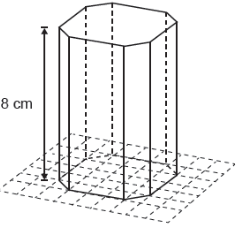
\includegraphics[width=7cm]{Extras/v3.png}
	\end{figure}

Qual é a medida do volume desse prisma?

\begin{enumerate}
\item 128 cm$^3$
\item 144 cm$^3$
\item 174 cm$^3$
\item 184 cm$^3$
\item 368 cm$^3$
\end{enumerate}

% ==============================================================

\item As dimensões de uma piscina olímpica são: 50 m de comprimento, 25 m de largura e 3 m de profundidade. O seu volume em m$^3$ é 

\begin{enumerate}
\item 7500 m$^3$. 
\item 3750 m$^3$. 
\item 1253 m$^3$. 
\item 175 m$^3$. 
\item 78 m$^3$.
\end{enumerate}

% ==============================================================

\item 75 litros de água foram colocados em um recipiente vazio, de forma cilíndrica, cujas medidas são: 25 cm de raio e 80 cm de altura. A quantidade de água colocada no recipiente é
Dados:

\begin{enumerate}
\item a metade da capacidade.
\item igual à capacidade.
\item maior que a capacidade.
\item um quinto da capacidade.
\item um terço da capacidade.
\end{enumerate}

% ==============================================================

\item Um pedaço cilíndrico de cano de 30 cm de comprimento e 10cm de diâmetro interno encontra-se na posição vertical e possui a parte interior vedada. Colocando-se 2 litros de água em seu interior, a água:

\begin{enumerate}
\item transborda.
\item ultrapassa o meio do cano.
\item Enche o cano até a borda.
\item Não chega ao meio do cano. 
\item Enche ao até o meio do cano. 
\end{enumerate}

% ==============================================================

\item Uma embalagem de talco de forma cilíndrica possui 15 centímetros de altura e base com 3 centímetros de raio. Qual é o volume máximo, em cm$^3$, de talco que essa embalagem comporta? 

\begin{enumerate}
\item  540 $\pi$
\item 180 $\pi$
\item 135 $\pi$
\item 90 $\pi$
\item 45 $\pi$
\end{enumerate}

% ==============================================================

\item 

	\begin{figure}[!htb]
	\center
	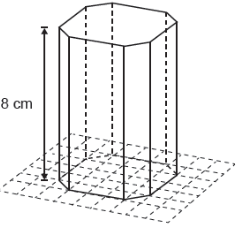
\includegraphics[width=7cm]{Extras/v3.png}
	\end{figure}


\begin{enumerate}
\item 
\end{enumerate}


% ==============================================================

\item 

	\begin{figure}[!htb]
	\center
	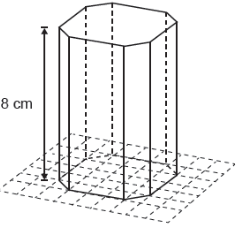
\includegraphics[width=7cm]{Extras/v3.png}
	\end{figure}


\begin{enumerate}
\item 
\end{enumerate}



% ==============================================================

\item 

	\begin{figure}[!htb]
	\center
	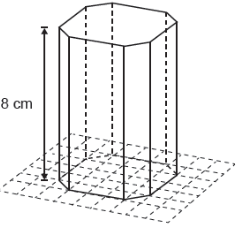
\includegraphics[width=7cm]{Extras/v3.png}
	\end{figure}


\begin{enumerate}
\item 
\end{enumerate}



% ==============================================================

\item 

	\begin{figure}[!htb]
	\center
	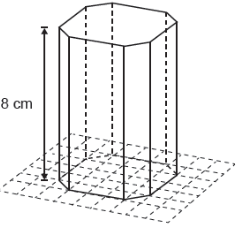
\includegraphics[width=7cm]{Extras/v3.png}
	\end{figure}


\begin{enumerate}
\item 
\end{enumerate}


% ==============================================================

\item 

	\begin{figure}[!htb]
	\center
	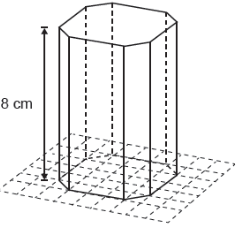
\includegraphics[width=7cm]{Extras/v3.png}
	\end{figure}


\begin{enumerate}
\item 
\end{enumerate}



\end{enumerate}
\end{document}